\documentclass[]{usiinfbachelorproject}
\usepackage{subfig}
\usepackage{caption}
\usepackage{subcaption}
\usepackage{float}
\captionsetup{labelfont={bf}}

\newcommand\subsubsection{\@startsection{subsubsection}{3}{\z@}%
                {-3.25ex\@plus -1ex \@minus -.2ex}%
                {1.5ex \@plus .2ex}%
                {\normalfont\normalsize\bfseries}}
\newcommand\paragraph{\@startsection{paragraph}{4}{\z@}%
                {3.25ex \@plus1ex \@minus.2ex}%
                {-1em}%
                {\normalfont\normalsize\bfseries}}
\author{Your Name}

\title{The Title}
\subtitle{The (optional) subtitle}
\versiondate{\today}
\begin{committee}
%With more than 1 advisor an error is raised...: only 1 advisor is allowed!
\advisor[Universit\`a della Svizzera Italiana, Switzerland]{Prof.}{AdvisorName}{AdvisorSurname}
%You can comment out  these lines if you don't have any assistant
\assistant[Universit\`a della Svizzera Italiana, Switzerland]{Title}{AssistantName1}{AssistanSurname1}
\assistant[Universit\`a della Svizzera Italiana, Switzerland]{Title}{AssistantName2}{AssistanSurname2}
\end{committee}


\abstract {
An abstract describing what the prospectus is all about. ``Omit needless words'' \cite{Stru1899a}: It should fit within the page without making the footer of the title page break the page --- otherwise what kind of abstract would it be?
}


\begin{document}
\maketitle

%%%%%%%%%%%%%%%%%%%%%%%%%
\section{Introduction}
\subsection{Motivation}

Big displays represent a widely used form of mass communication in almost all public places such as squares, subways and schools. They are used in a passive way by pushing un-targeted information, mostly advertisements, to the audience; enslaved by an bidirectional visible communication without any way to personalise the screen's content.

This lack of aimed content bring to a uniqueness of the display's message, since it must be equal for everyone. We can see the abuse of this strategy in the following pictures showing two of the world's biggest squares that are invaded by static, brightly, unavoidable, content from the huge displays.
\begin{figure}[H]
  \centering
  \subfloat[]{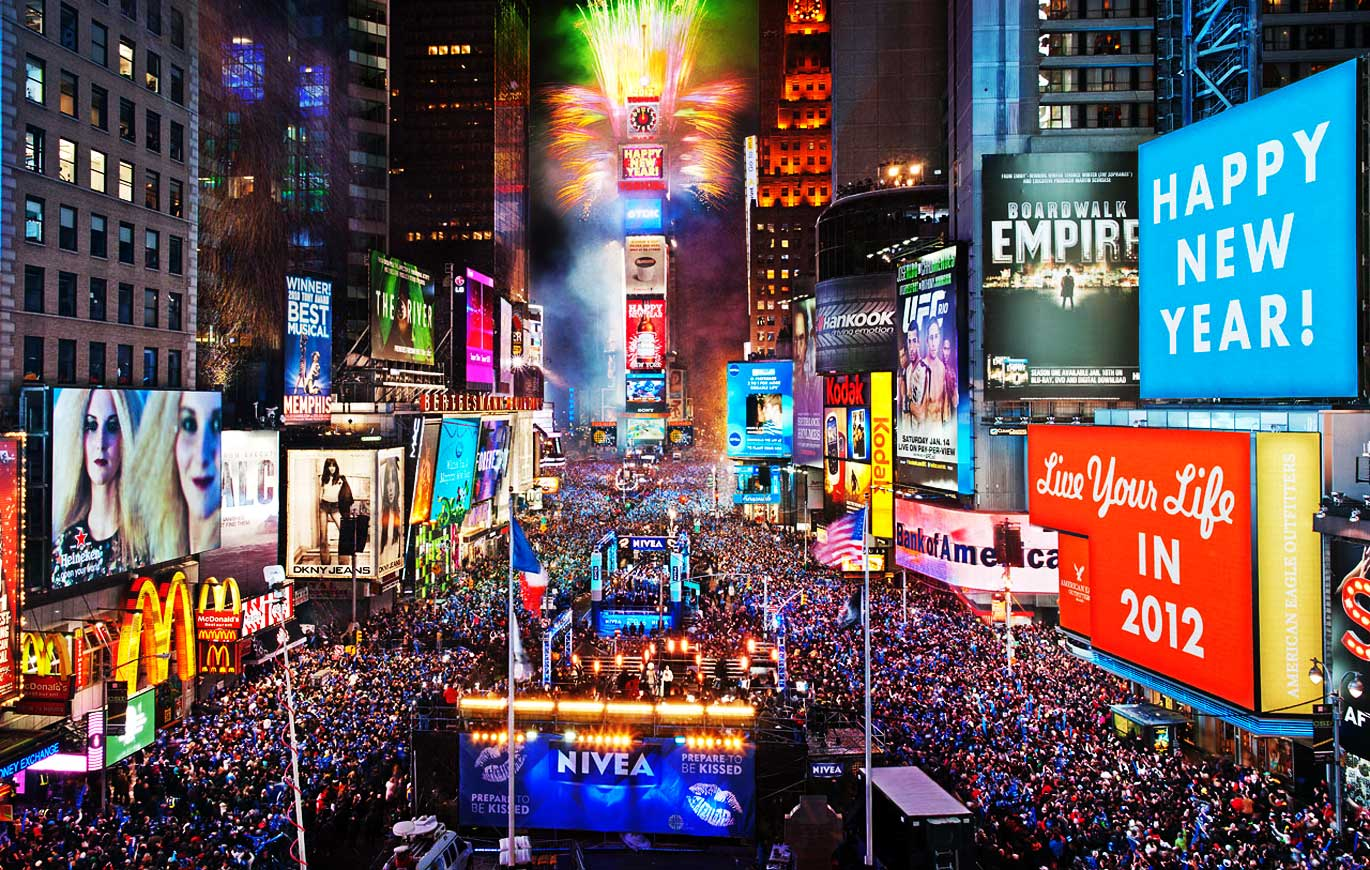
\includegraphics[width=0.4\textwidth]{./images/new_york_displays.jpg}}
  \hfill
  \subfloat[]{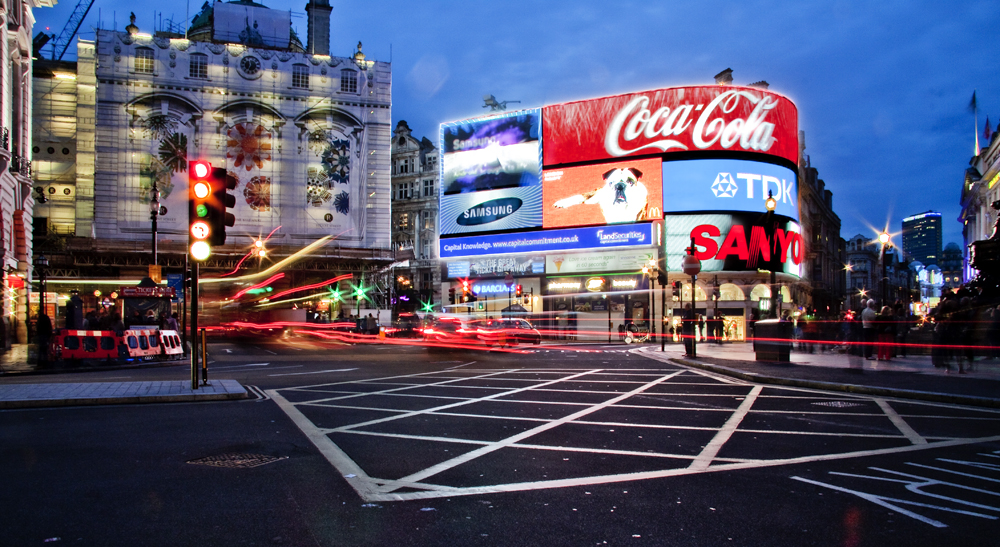
\includegraphics[width=0.45\textwidth]{./images/piccadilly_displays.jpg}}
\end{figure} 

We can see how such devices make a big impact on a town's shape, they chan it's look, colours and feel without adding anything useful. If we look carefully in the pictures we can notice that the only content showed is advertisement. The choice of content is not related directly to the technology, even before the display were available in such dimensions. In the following picture showing \emph{New York} in the early 60s we can notice the exactly same advertisement, even from the same companies, that is showed today. Therefore, what is the utility of using displays instead of posters, you may ask.

\begin{figure}[H]
  \centering
  \subfloat[]{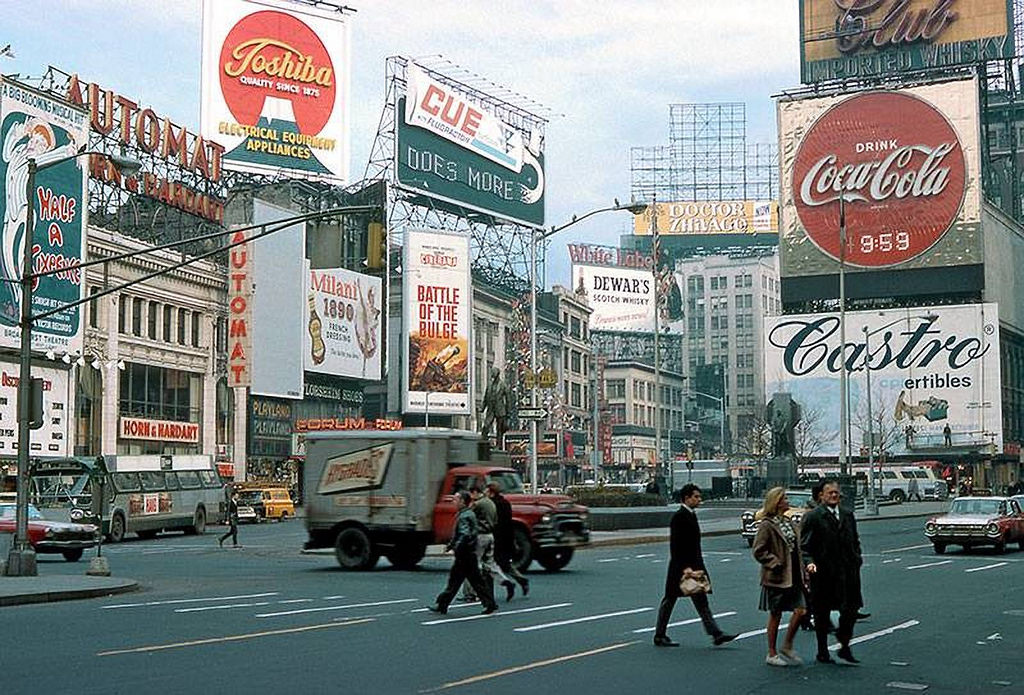
\includegraphics[width=0.4\textwidth]{./images/new_york_posters.jpg}}
\end{figure} 
Since the message from the display is shared, or forced, to everyone, it seems logic thinking that everyone should share the screen, but that is not the case.

A unified message cause a certainly reduction of the screen's utility and purpose, making it, as we stated before, a full passive element. An other example of a badly use of displays may be the ones in the Milan \emph{Stazione Centrale}, showed in the following picture.
% add picture
They are used only to show publicity from the TV's channels loosing all the power that such devices embraces. Would be nice to just walk close to one of these and see our train schedules? Obviously yes. 


\subsection{Goal}

Our goal is to create a bi-lateral channel with the screen: the user must be able to quickly filter the information that he needs in just few seconds without being shelled by tons of useless brands and images. As it is deeply described in the next sections, in our topology, the user is the active trigger that push and pull it's personal content into and from the screen. This personalised information can be showed by just walking to the display thanks to proximity sensors such as bluetooth beacons; this allow a non blocking information flow where only the relevant content is target to the interested user at the right time.
\\
\\
The information should be pertinent and \emph{fast}, it must be easy for the user to enter the topology and become a part of it without loosing any time. Tons of studied shows the connection between poorly user interaction and high learning curve. Since we are addressing a endless mass of people, our application must be easy to start with and addressable, for those we used smart phones as mainly platform
% ADD SOMETHING talk abou speed and user interaface with the smartphone

By doing that we completly transform a tool, such as a display, into a new one, a better one.
% say something of how software can change hardware an it is the main layer
\section{Topology}
In this section we describe in detail the whole project design, bottom-up. Starting by a briefly description of how we structure all the parts.
\subsection{Topology Architecture}
% INTRODUCTION
Design a working system is never easy. It has to logically mimic the answer to the problem we are trying to solve.
\\
\\
We are looking for a scalable system where the user, identifier as an active entry, pull and push his information to the display. With \emph{scalable} we means that it does not directly depends on the number of application, or \emph{sercices}, our network exposes. Also the display number must be irrelevant, the system has to work with $n$ display and $m$ application without any changing in the core.
% GENERAL OVERVIEW
For such reasons we adopted a \emph{Micro Services} architecture where each element can be removed without effecting the intigrity of the system. Services communicate using either synchronous protocols such as HTTP/REST; thus can be developed and deployed independently of one another. Each service has its own database in order to be decoupled from other services. In our project we deployed all the services on the same server, but in a real world application they are usually physical separated.
\\
\\
 We started by \emph{abstracting} the applications layers, that for now, it is seen as a single entity. This layers provided a common interface for pull/push personalization.
 All the active logic of the network is handled by another Micro Service, called \emph{Tacita}, that links display, application and users. It's responsibility is to be the glue between the application layer and the other elements by storing users informations, display's state and available applications.
% TALK about the system that must be anynimous 

\subsection{Topology Elements}
\subsubsection{General Overview}

We talked superfically of the elements of our Topology: it is time to deeply describe them one per one. We start from the most important one: The User  
\subsubsection{User}

The User has a fully active role, he is the trigger of the whole system; without him, the network has not reason to exits. He uses his smartphone in order to access the front-end application exposed by our back-end micro services through the \emph{Tacita} platform.

By using it the User can selects his custom settings in order to quickly identify his information on the screens. For instance, a favourite colour can be used for such pourpose gaining, at the same time, anonymity, and a quick way to identify his personalized content by just watching the screen. Thus only the targeted client knows which are his information. The app will be deeply analised into the next sections, but, from a user point of view, it is the door to access the array of services.

We talked about the User as a \emph{trigger}, it means that, with his physical being, it \emph{triggers} actions; actions that are universally recognizable by our topology. In our system we use bluetooth beacon near the screens to map them in the space, and, thanks to the smartphone application, we can detect the user walking into the trigger range and show the personalized content into the screen at the right time. 

Timing is a fundamental variable in our ecosystem, if the actions is not handled at the correct time the topology is unreliable and the display is not used correctly, or, not used at all. 
\subsubsection{Display}

Display represent our \emph{tabula rasa} in which we can out a wide array of applications can be showed. By itself it is a \emph{passive} entry, but, combined to the User becomes the second \emph{active} element of our topology. The two way communication channel between them is created thanks to web socket and bluetooth beacon. When a user walk next to a screen a bluetooth sensor notify the \emph{Tacita} application that there is a screen, such information is used to push into a web socket, in which the display is connected, the user unique identifier. As soon as it is received, a request to the running application is made in order to get the preferences and showed them; since we are using a common \emph{interface} in the Application layer, each of them expose the same structure to perform CRUD operations.
In our design we decide to only send the minimum amount of data that the display can need. Assuming a user walk near display one, this the notification pushed into the socked:

% ADD JSON

As you can see, we just send the user's id, the display's id and the custom color, by doing that, the display can be completely independent.

Since a touch interface is used in our project the communication channel can be enlarge by also allowing the user to click in order to reveal some content, for example, a specific bus number.

% add photo of the user display interaction
 We choose a web interface as mainly platform for our display since it is easy to maintain ad  scale; a full section about the web techonologies used can be founded in 2.4. Briefly, a website is show on the big screens and, thank to a socket connection, real-time changes can be displayed.
\subsection{Topology Interactions}
\subsection{Topology Technologies}
\subsection{Topology Scalability}
\section{Design}
\subsection{Back-end}
\subsection{Front-end}
\section{Conclusion}
\section{Acknowledges}

\newpage



%%%%%
\bibliographystyle{abbrv}
\bibliography{references}
\end{document}